\documentclass[twoside]{book}

% Packages required by doxygen
\usepackage{fixltx2e}
\usepackage{calc}
\usepackage{doxygen}
\usepackage[export]{adjustbox} % also loads graphicx
\usepackage{graphicx}
\usepackage[utf8]{inputenc}
\usepackage{makeidx}
\usepackage{multicol}
\usepackage{multirow}
\PassOptionsToPackage{warn}{textcomp}
\usepackage{textcomp}
\usepackage[nointegrals]{wasysym}
\usepackage[table]{xcolor}

% Font selection
\usepackage[T1]{fontenc}
\usepackage[scaled=.90]{helvet}
\usepackage{courier}
\usepackage{amssymb}
\usepackage{sectsty}
\renewcommand{\familydefault}{\sfdefault}
\allsectionsfont{%
  \fontseries{bc}\selectfont%
  \color{darkgray}%
}
\renewcommand{\DoxyLabelFont}{%
  \fontseries{bc}\selectfont%
  \color{darkgray}%
}
\newcommand{\+}{\discretionary{\mbox{\scriptsize$\hookleftarrow$}}{}{}}

% Page & text layout
\usepackage{geometry}
\geometry{%
  a4paper,%
  top=2.5cm,%
  bottom=2.5cm,%
  left=2.5cm,%
  right=2.5cm%
}
\tolerance=750
\hfuzz=15pt
\hbadness=750
\setlength{\emergencystretch}{15pt}
\setlength{\parindent}{0cm}
\setlength{\parskip}{3ex plus 2ex minus 2ex}
\makeatletter
\renewcommand{\paragraph}{%
  \@startsection{paragraph}{4}{0ex}{-1.0ex}{1.0ex}{%
    \normalfont\normalsize\bfseries\SS@parafont%
  }%
}
\renewcommand{\subparagraph}{%
  \@startsection{subparagraph}{5}{0ex}{-1.0ex}{1.0ex}{%
    \normalfont\normalsize\bfseries\SS@subparafont%
  }%
}
\makeatother

% Headers & footers
\usepackage{fancyhdr}
\pagestyle{fancyplain}
\fancyhead[LE]{\fancyplain{}{\bfseries\thepage}}
\fancyhead[CE]{\fancyplain{}{}}
\fancyhead[RE]{\fancyplain{}{\bfseries\leftmark}}
\fancyhead[LO]{\fancyplain{}{\bfseries\rightmark}}
\fancyhead[CO]{\fancyplain{}{}}
\fancyhead[RO]{\fancyplain{}{\bfseries\thepage}}
\fancyfoot[LE]{\fancyplain{}{}}
\fancyfoot[CE]{\fancyplain{}{}}
\fancyfoot[RE]{\fancyplain{}{\bfseries\scriptsize Generated by Doxygen }}
\fancyfoot[LO]{\fancyplain{}{\bfseries\scriptsize Generated by Doxygen }}
\fancyfoot[CO]{\fancyplain{}{}}
\fancyfoot[RO]{\fancyplain{}{}}
\renewcommand{\footrulewidth}{0.4pt}
\renewcommand{\chaptermark}[1]{%
  \markboth{#1}{}%
}
\renewcommand{\sectionmark}[1]{%
  \markright{\thesection\ #1}%
}

% Indices & bibliography
\usepackage{natbib}
\usepackage[titles]{tocloft}
\setcounter{tocdepth}{3}
\setcounter{secnumdepth}{5}
\makeindex

% Hyperlinks (required, but should be loaded last)
\usepackage{ifpdf}
\ifpdf
  \usepackage[pdftex,pagebackref=true]{hyperref}
\else
  \usepackage[ps2pdf,pagebackref=true]{hyperref}
\fi
\hypersetup{%
  colorlinks=true,%
  linkcolor=blue,%
  citecolor=blue,%
  unicode%
}

% Custom commands
\newcommand{\clearemptydoublepage}{%
  \newpage{\pagestyle{empty}\cleardoublepage}%
}

\usepackage{caption}
\captionsetup{labelsep=space,justification=centering,font={bf},singlelinecheck=off,skip=4pt,position=top}

%===== C O N T E N T S =====

\begin{document}

% Titlepage & ToC
\hypersetup{pageanchor=false,
             bookmarksnumbered=true,
             pdfencoding=unicode
            }
\pagenumbering{alph}
\begin{titlepage}
\vspace*{7cm}
\begin{center}%
{\Large Bandit\+P\+AM }\\
\vspace*{1cm}
{\large Generated by Doxygen 1.8.13}\\
\end{center}
\end{titlepage}
\clearemptydoublepage
\pagenumbering{roman}
\tableofcontents
\clearemptydoublepage
\pagenumbering{arabic}
\hypersetup{pageanchor=true}

%--- Begin generated contents ---
\chapter{Bandit\+P\+AM\+: Almost Linear-\/\+Time k-\/\+Medoids Clustering}
\label{index}\hypertarget{index}{}This repo contains a high-\/performance implementation of Bandit\+P\+AM from \href{https://arxiv.org/abs/2006.06856}{\tt https\+://arxiv.\+org/abs/2006.\+06856}. The code can be called directly from Python or C++.

If you use this software, please cite\+:

Mo Tiwari, Martin Jinye Zhang, James Mayclin, Sebastian Thrun, Chris Piech, Ilan Shomorony. \char`\"{}\+Bandit-\/\+P\+A\+M\+: Almost Linear Time k-\/medoids Clustering via Multi-\/\+Armed Bandits\char`\"{} Neural Information Processing Systems (Neur\+I\+PS) 2020.


\begin{DoxyCode}
@inproceedings\{BanditPAM,
  title=\{Bandit-PAM: Almost Linear Time k-medoids Clustering via Multi-Armed Bandits\},
  author=\{Tiwari, Mo and Zhang, Martin J and Mayclin, James and Thrun, Sebastian and Piech, Chris and
       Shomorony, Ilan\},
  booktitle=\{Advances in Neural Information Processing Systems\},
  pages=\{368--374\}, #TODO: Fix this
  year=\{2020\}
\}
\end{DoxyCode}


\section*{Python Quickstart}

\subsection*{Install the repo and its dependencies\+:}


\begin{DoxyCode}
/BanditPAM/: pip install -r requirements.txt
/BanditPAM/: sudo pip install .
\end{DoxyCode}


\subsubsection*{Example 1\+: Synthetic data from a Gaussian Mixture Model}


\begin{DoxyCode}
from BanditPAM import KMedoids
import numpy as np
import matplotlib.pyplot as plt

# Generate data from a Gaussian Mixture Model with the given means:
np.random.seed(0)
n\_per\_cluster = 40
means = np.array([[0,0], [-5,5], [5,5]])
X = np.vstack([np.random.randn(n\_per\_cluster, 2) + mu for mu in means])

# Fit the data with BanditPAM:
kmed = KMedoids(n\_medoids = 3, algorithm = "BanditPAM")
# Writes results to gmm\_log
kmed.fit(X, 'L2', 3, "gmm\_log")

# Visualize the data and the medoids:
for p\_idx, point in enumerate(X):
    if p\_idx in map(int, kmed.final\_medoids):
        plt.scatter(X[p\_idx, 0], X[p\_idx, 1], color='red', s = 40)
    else:
        plt.scatter(X[p\_idx, 0], X[p\_idx, 1], color='blue', s = 10)
plt.show()
\end{DoxyCode}




\subsubsection*{Example 2\+: M\+N\+I\+ST and its medoids visualized via t-\/\+S\+NE}


\begin{DoxyCode}
from BanditPAM import KMedoids
import numpy as np
import pandas as pd
import matplotlib.pyplot as plt
from sklearn.manifold import TSNE

# Load the 1000-point subset of MNIST and calculate its t-SNE embeddings for visualization:
X = pd.read\_csv('data/MNIST-1k.csv', sep=' ', header=None).to\_numpy()
X\_tsne = TSNE(n\_components = 2).fit\_transform(X)

# Fit the data with BanditPAM:
kmed = KMedoids(n\_medoids = 10, algorithm = "BanditPAM")
kmed.fit(X, 'L2', 10, "mnist\_log")

# Visualize the data and the medoids via t-SNE:
for p\_idx, point in enumerate(X):
    if p\_idx in map(int, kmed.final\_medoids):
        plt.scatter(X\_tsne[p\_idx, 0], X\_tsne[p\_idx, 1], color='red', s = 40)
    else:
        plt.scatter(X\_tsne[p\_idx, 0], X\_tsne[p\_idx, 1], color='blue', s = 5)
plt.show()
\end{DoxyCode}
 The corresponding logfile for this run, {\ttfamily mnist\+\_\+log}, will contain the run\textquotesingle{}s results and additional statistics in a format that can be easily read into json.

\subsection*{Building the C++ executable from source}

Please note that it is not necessary to build the C++ executable from source to use the Python code above. However, if you would like to use the C++ executable directly, follow the instructions below.

\subsubsection*{Option 1\+: Building with Docker}

We highly recommend building using Docker. Once you have Docker installed and the Docker Daemon is running, run the following commands\+:


\begin{DoxyCode}
/BanditPAM$ chmod +x env\_setup.sh
/BanditPAM$ ./env\_setup.sh
/BanditPAM$ ./run\_docker.sh
\end{DoxyCode}


which will start a Docker instance with the necessary dependencies. Then\+:


\begin{DoxyCode}
/BanditPAM$ mkdir build && cd build
/BanditPAM/build$ cmake .. && make
\end{DoxyCode}


This will create an executable named {\ttfamily Bandit\+P\+AM} in {\ttfamily Bandit\+P\+A\+M/build/src}.

\subsubsection*{Option 2\+: Installing Requirements and Building Directly}

Building this repository requires three external requirements\+:
\begin{DoxyItemize}
\item Cmake $>$= 3.\+17
\item Armadillo $>$= 9.\+7, \href{http://arma.sourceforge.net/download.html}{\tt http\+://arma.\+sourceforge.\+net/download.\+html}
\item Open\+MP $>$= 2.\+5, \href{https://www.openmp.org/resources/openmp-compilers-tools/}{\tt https\+://www.\+openmp.\+org/resources/openmp-\/compilers-\/tools/} (Open\+MP is supported by default on most Linux platforms, and can be downloaded through homebrew on macs.)
\item C\+A\+R\+MA $>$= 0.\+3.\+0, \href{https://github.com/RUrlus/carma}{\tt https\+://github.\+com/\+R\+Urlus/carma}
\end{DoxyItemize}

Ensure all the requirements above are installed and then run\+:


\begin{DoxyCode}
/BanditPAM$ mkdir build && cd build
/BanditPAM/build$ cmake .. && make
\end{DoxyCode}


This will create an executable named {\ttfamily Bandit\+P\+AM} in {\ttfamily Bandit\+P\+A\+M/build/src}.

\subsection*{Usage}

Once the executable has been built, it can be invoked with\+: 
\begin{DoxyCode}
/BanditPAM/build/src/BanditPAM -f [path/to/input.csv] -k [number of clusters] -v [verbosity level]
\end{DoxyCode}



\begin{DoxyItemize}
\item {\ttfamily -\/f} is mandatory and specifies the path to the dataset
\item {\ttfamily -\/k} is mandatory and specifies the number of clusters with which to fit the data
\item {\ttfamily -\/v} is optional and specifies the verbosity level.
\end{DoxyItemize}

For example, if you ran {\ttfamily ./env\+\_\+setup.sh} and downloaded the M\+N\+I\+ST dataset, you could run\+:


\begin{DoxyCode}
/BanditPAM/build/src/BanditPAM -f ../data/MNIST-1k.csv -k 10
\end{DoxyCode}
 
\chapter{Hierarchical Index}
\section{Class Hierarchy}
This inheritance list is sorted roughly, but not completely, alphabetically\+:\begin{DoxyCompactList}
\item K\+Medoids\begin{DoxyCompactList}
\item \contentsline{section}{K\+Meds\+Wrapper}{\pageref{classKMedsWrapper}}{}
\end{DoxyCompactList}
\end{DoxyCompactList}

\chapter{Class Index}
\doxysection{Class List}
Here are the classes, structs, unions and interfaces with brief descriptions\+:\begin{DoxyCompactList}
\item\contentsline{section}{\mbox{\hyperlink{classkm_1_1BanditPAM}{km\+::\+Bandit\+PAM}} \\*Contains all necessary \mbox{\hyperlink{classkm_1_1BanditPAM}{Bandit\+PAM}} functions }{\pageref{classkm_1_1BanditPAM}}{}
\item\contentsline{section}{\mbox{\hyperlink{classkm_1_1FastPAM1}{km\+::\+Fast\+PAM1}} \\*Class implementation for \mbox{\hyperlink{classkm_1_1FastPAM1}{Fast\+PAM1}} algorithm }{\pageref{classkm_1_1FastPAM1}}{}
\item\contentsline{section}{\mbox{\hyperlink{classkm_1_1KMedoids}{km\+::\+KMedoids}} \\*Class implementation for running \mbox{\hyperlink{classkm_1_1KMedoids}{KMedoids}} methods }{\pageref{classkm_1_1KMedoids}}{}
\item\contentsline{section}{\mbox{\hyperlink{classkm_1_1KMedoidsWrapper}{km\+::\+KMedoids\+Wrapper}} \\*Python wrapper for \mbox{\hyperlink{classkm_1_1KMedoids}{KMedoids}} class }{\pageref{classkm_1_1KMedoidsWrapper}}{}
\item\contentsline{section}{\mbox{\hyperlink{classkm_1_1PAM}{km\+::\+PAM}} \\*Class implementation for \mbox{\hyperlink{classkm_1_1PAM}{PAM}} algorithm }{\pageref{classkm_1_1PAM}}{}
\end{DoxyCompactList}

\chapter{File Index}
\section{File List}
Here is a list of all documented files with brief descriptions\+:\begin{DoxyCompactList}
\item\contentsline{section}{/home/esfrankel/\+Desktop/\+Bandit\+P\+A\+M/src/\hyperlink{kmedoids__ucb_8cpp}{kmedoids\+\_\+ucb.\+cpp} }{\pageref{kmedoids__ucb_8cpp}}{}
\item\contentsline{section}{/home/esfrankel/\+Desktop/\+Bandit\+P\+A\+M/src/\hyperlink{kmeds__pywrapper_8cpp}{kmeds\+\_\+pywrapper.\+cpp} }{\pageref{kmeds__pywrapper_8cpp}}{}
\item\contentsline{section}{/home/esfrankel/\+Desktop/\+Bandit\+P\+A\+M/src/\hyperlink{main_8cpp}{main.\+cpp} }{\pageref{main_8cpp}}{}
\end{DoxyCompactList}

\chapter{Class Documentation}
\hypertarget{classKMedoids}{}\section{K\+Medoids Class Reference}
\label{classKMedoids}\index{K\+Medoids@{K\+Medoids}}


{\ttfamily \#include $<$kmedoids\+\_\+ucb.\+hpp$>$}



Inheritance diagram for K\+Medoids\+:\nopagebreak
\begin{figure}[H]
\begin{center}
\leavevmode
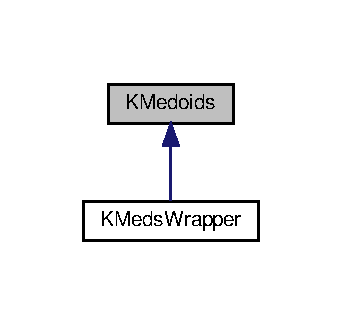
\includegraphics[width=164pt]{classKMedoids__inherit__graph}
\end{center}
\end{figure}
\subsection*{Public Member Functions}
\begin{DoxyCompactItemize}
\item 
\hyperlink{classKMedoids_aa94dfc65454f847af5d08a2d7b816bb4}{K\+Medoids} (int n\+\_\+medoids=5, std\+::string algorithm=\char`\"{}Bandit\+P\+AM\char`\"{}, int verbosity=0, int max\+\_\+iter=1000, std\+::string log\+Filename=\char`\"{}K\+Medoids\+Logfile\char`\"{})
\item 
\mbox{\Hypertarget{classKMedoids_a3d05d453ee8c395102ac9d20c91a9a12}\label{classKMedoids_a3d05d453ee8c395102ac9d20c91a9a12}} 
{\bfseries K\+Medoids} (const \hyperlink{classKMedoids}{K\+Medoids} \&kmed)
\item 
\hyperlink{classKMedoids_a82710100b6fb5820c10bc3f796ed62ff}{$\sim$\+K\+Medoids} ()
\item 
void \hyperlink{classKMedoids_a65760033bcae8de418d350c6fc4981da}{set\+N\+Medoids} (int k)
\item 
void \hyperlink{classKMedoids_a70de4f833f95a0256cce42284ebb3d48}{set\+Log\+Filename} (std\+::string l)
\item 
void \hyperlink{classKMedoids_ab68f7ee100ab2a15bc6ee0ba28f128ba}{fit} (arma\+::mat input\+\_\+data, std\+::string loss)
\item 
arma\+::rowvec \hyperlink{classKMedoids_a26aa9827d2541626d959dc984f0f9bcb}{get\+Medoids\+Final} ()
\item 
arma\+::rowvec \hyperlink{classKMedoids_a54370d8d0f5c500f5deb859a9eab891c}{get\+Medoids\+Build} ()
\item 
arma\+::rowvec \hyperlink{classKMedoids_a89474787892880381e4d0282de541d03}{get\+Labels} ()
\item 
void \hyperlink{classKMedoids_ab442bf7198be7a48a7eb5901ac7ca571}{set\+Loss\+Fn} (std\+::string loss)
\item 
void \hyperlink{classKMedoids_af5b9331755cd049afb05af8ecee3aeb5}{check\+Algorithm} (std\+::string algorithm)
\item 
int \hyperlink{classKMedoids_a2c8d55468ebe909229ea7bcdb50e8351}{get\+Steps} ()
\end{DoxyCompactItemize}
\subsection*{Public Attributes}
\begin{DoxyCompactItemize}
\item 
\mbox{\Hypertarget{classKMedoids_a3365e728fd524c0be2fbab0b58e3a4cd}\label{classKMedoids_a3365e728fd524c0be2fbab0b58e3a4cd}} 
int {\bfseries n\+\_\+medoids}
\item 
\mbox{\Hypertarget{classKMedoids_a3cf57e612442072fb377b1714fc5e12e}\label{classKMedoids_a3cf57e612442072fb377b1714fc5e12e}} 
std\+::string {\bfseries log\+Filename}
\end{DoxyCompactItemize}


\subsection{Detailed Description}
\hyperlink{classKMedoids}{K\+Medoids} class. Creates a \hyperlink{classKMedoids}{K\+Medoids} object that can be used to find the medoids for a particular set of input data.


\begin{DoxyParams}{Parameters}
{\em n\+\_\+medoids} & Number of medoids to identify \\
\hline
{\em algorithm} & Algorithm to use to find medoids; options are \char`\"{}\+Bandit\+P\+A\+M\char`\"{} for this paper\textquotesingle{}s iplementation, or \char`\"{}naive\char`\"{} to use the naive method \\
\hline
{\em verbosity} & Verbosity of the algorithm, 0 will have no log file emitted, 1 will emit a log file \\
\hline
{\em max\+\_\+iter} & The maximum number of iterations to run the algorithm for \\
\hline
{\em log\+Filename} & The name of the output log file \\
\hline
\end{DoxyParams}


\subsection{Constructor \& Destructor Documentation}
\mbox{\Hypertarget{classKMedoids_aa94dfc65454f847af5d08a2d7b816bb4}\label{classKMedoids_aa94dfc65454f847af5d08a2d7b816bb4}} 
\index{K\+Medoids@{K\+Medoids}!K\+Medoids@{K\+Medoids}}
\index{K\+Medoids@{K\+Medoids}!K\+Medoids@{K\+Medoids}}
\subsubsection{\texorpdfstring{K\+Medoids()}{KMedoids()}}
{\footnotesize\ttfamily K\+Medoids\+::\+K\+Medoids (\begin{DoxyParamCaption}\item[{int}]{n\+\_\+medoids = {\ttfamily 5},  }\item[{std\+::string}]{algorithm = {\ttfamily \char`\"{}BanditPAM\char`\"{}},  }\item[{int}]{verbosity = {\ttfamily 0},  }\item[{int}]{max\+\_\+iter = {\ttfamily 1000},  }\item[{std\+::string}]{log\+Filename = {\ttfamily \char`\"{}KMedoidsLogfile\char`\"{}} }\end{DoxyParamCaption})}

\hyperlink{classKMedoids}{K\+Medoids} class. Creates a \hyperlink{classKMedoids}{K\+Medoids} object that can be used to find the medoids for a particular set of input data.


\begin{DoxyParams}{Parameters}
{\em n\+\_\+medoids} & Number of medoids to identify \\
\hline
{\em algorithm} & Algorithm to use to find medoids; options are \char`\"{}\+Bandit\+P\+A\+M\char`\"{} for this paper\textquotesingle{}s iplementation, or \char`\"{}naive\char`\"{} to use the naive method \\
\hline
{\em verbosity} & Verbosity of the algorithm, 0 will have no log file emitted, 1 will emit a log file \\
\hline
{\em max\+\_\+iter} & The maximum number of iterations to run the algorithm for \\
\hline
{\em log\+Filename} & The name of the output log file \\
\hline
\end{DoxyParams}
\mbox{\Hypertarget{classKMedoids_a82710100b6fb5820c10bc3f796ed62ff}\label{classKMedoids_a82710100b6fb5820c10bc3f796ed62ff}} 
\index{K\+Medoids@{K\+Medoids}!````~K\+Medoids@{$\sim$\+K\+Medoids}}
\index{````~K\+Medoids@{$\sim$\+K\+Medoids}!K\+Medoids@{K\+Medoids}}
\subsubsection{\texorpdfstring{$\sim$\+K\+Medoids()}{~KMedoids()}}
{\footnotesize\ttfamily K\+Medoids\+::$\sim$\+K\+Medoids (\begin{DoxyParamCaption}{ }\end{DoxyParamCaption})}

This function is the destructor for the \hyperlink{classKMedoids}{K\+Medoids} class. 

\subsection{Member Function Documentation}
\mbox{\Hypertarget{classKMedoids_af5b9331755cd049afb05af8ecee3aeb5}\label{classKMedoids_af5b9331755cd049afb05af8ecee3aeb5}} 
\index{K\+Medoids@{K\+Medoids}!check\+Algorithm@{check\+Algorithm}}
\index{check\+Algorithm@{check\+Algorithm}!K\+Medoids@{K\+Medoids}}
\subsubsection{\texorpdfstring{check\+Algorithm()}{checkAlgorithm()}}
{\footnotesize\ttfamily void K\+Medoids\+::check\+Algorithm (\begin{DoxyParamCaption}\item[{std\+::string}]{algorithm }\end{DoxyParamCaption})}

This function sets the algorithm the \hyperlink{classKMedoids}{K\+Medoids} object will use \mbox{\Hypertarget{classKMedoids_ab68f7ee100ab2a15bc6ee0ba28f128ba}\label{classKMedoids_ab68f7ee100ab2a15bc6ee0ba28f128ba}} 
\index{K\+Medoids@{K\+Medoids}!fit@{fit}}
\index{fit@{fit}!K\+Medoids@{K\+Medoids}}
\subsubsection{\texorpdfstring{fit()}{fit()}}
{\footnotesize\ttfamily void K\+Medoids\+::fit (\begin{DoxyParamCaption}\item[{arma\+::mat}]{input\+\_\+data,  }\item[{std\+::string}]{loss }\end{DoxyParamCaption})}

This is the main function of the \hyperlink{classKMedoids}{K\+Medoids} object\+: this finds the build and swap medoids for the desired data


\begin{DoxyParams}{Parameters}
{\em input\+\_\+data} & Input data to find the medoids of \\
\hline
{\em loss} & The loss function used during medoid computation \\
\hline
\end{DoxyParams}
\mbox{\Hypertarget{classKMedoids_a89474787892880381e4d0282de541d03}\label{classKMedoids_a89474787892880381e4d0282de541d03}} 
\index{K\+Medoids@{K\+Medoids}!get\+Labels@{get\+Labels}}
\index{get\+Labels@{get\+Labels}!K\+Medoids@{K\+Medoids}}
\subsubsection{\texorpdfstring{get\+Labels()}{getLabels()}}
{\footnotesize\ttfamily arma\+::rowvec K\+Medoids\+::get\+Labels (\begin{DoxyParamCaption}{ }\end{DoxyParamCaption})}

This function returns the labels/medoids assignments for each datapoint after the final medoids are identified. \mbox{\Hypertarget{classKMedoids_a54370d8d0f5c500f5deb859a9eab891c}\label{classKMedoids_a54370d8d0f5c500f5deb859a9eab891c}} 
\index{K\+Medoids@{K\+Medoids}!get\+Medoids\+Build@{get\+Medoids\+Build}}
\index{get\+Medoids\+Build@{get\+Medoids\+Build}!K\+Medoids@{K\+Medoids}}
\subsubsection{\texorpdfstring{get\+Medoids\+Build()}{getMedoidsBuild()}}
{\footnotesize\ttfamily arma\+::rowvec K\+Medoids\+::get\+Medoids\+Build (\begin{DoxyParamCaption}{ }\end{DoxyParamCaption})}

This function returns the build medoids for a \hyperlink{classKMedoids}{K\+Medoids} object. \mbox{\Hypertarget{classKMedoids_a26aa9827d2541626d959dc984f0f9bcb}\label{classKMedoids_a26aa9827d2541626d959dc984f0f9bcb}} 
\index{K\+Medoids@{K\+Medoids}!get\+Medoids\+Final@{get\+Medoids\+Final}}
\index{get\+Medoids\+Final@{get\+Medoids\+Final}!K\+Medoids@{K\+Medoids}}
\subsubsection{\texorpdfstring{get\+Medoids\+Final()}{getMedoidsFinal()}}
{\footnotesize\ttfamily arma\+::rowvec K\+Medoids\+::get\+Medoids\+Final (\begin{DoxyParamCaption}{ }\end{DoxyParamCaption})}

This function returns the final medoids for a \hyperlink{classKMedoids}{K\+Medoids} object. \mbox{\Hypertarget{classKMedoids_a2c8d55468ebe909229ea7bcdb50e8351}\label{classKMedoids_a2c8d55468ebe909229ea7bcdb50e8351}} 
\index{K\+Medoids@{K\+Medoids}!get\+Steps@{get\+Steps}}
\index{get\+Steps@{get\+Steps}!K\+Medoids@{K\+Medoids}}
\subsubsection{\texorpdfstring{get\+Steps()}{getSteps()}}
{\footnotesize\ttfamily int K\+Medoids\+::get\+Steps (\begin{DoxyParamCaption}{ }\end{DoxyParamCaption})}

This function returns the number of swap steps that took place during the computation \mbox{\Hypertarget{classKMedoids_a70de4f833f95a0256cce42284ebb3d48}\label{classKMedoids_a70de4f833f95a0256cce42284ebb3d48}} 
\index{K\+Medoids@{K\+Medoids}!set\+Log\+Filename@{set\+Log\+Filename}}
\index{set\+Log\+Filename@{set\+Log\+Filename}!K\+Medoids@{K\+Medoids}}
\subsubsection{\texorpdfstring{set\+Log\+Filename()}{setLogFilename()}}
{\footnotesize\ttfamily void K\+Medoids\+::set\+Log\+Filename (\begin{DoxyParamCaption}\item[{std\+::string}]{l }\end{DoxyParamCaption})}

This function sets the log file name \mbox{\Hypertarget{classKMedoids_ab442bf7198be7a48a7eb5901ac7ca571}\label{classKMedoids_ab442bf7198be7a48a7eb5901ac7ca571}} 
\index{K\+Medoids@{K\+Medoids}!set\+Loss\+Fn@{set\+Loss\+Fn}}
\index{set\+Loss\+Fn@{set\+Loss\+Fn}!K\+Medoids@{K\+Medoids}}
\subsubsection{\texorpdfstring{set\+Loss\+Fn()}{setLossFn()}}
{\footnotesize\ttfamily void K\+Medoids\+::set\+Loss\+Fn (\begin{DoxyParamCaption}\item[{std\+::string}]{loss }\end{DoxyParamCaption})}

This function sets the loss function the \hyperlink{classKMedoids}{K\+Medoids} object will use \mbox{\Hypertarget{classKMedoids_a65760033bcae8de418d350c6fc4981da}\label{classKMedoids_a65760033bcae8de418d350c6fc4981da}} 
\index{K\+Medoids@{K\+Medoids}!set\+N\+Medoids@{set\+N\+Medoids}}
\index{set\+N\+Medoids@{set\+N\+Medoids}!K\+Medoids@{K\+Medoids}}
\subsubsection{\texorpdfstring{set\+N\+Medoids()}{setNMedoids()}}
{\footnotesize\ttfamily void K\+Medoids\+::set\+N\+Medoids (\begin{DoxyParamCaption}\item[{int}]{k }\end{DoxyParamCaption})}

This function sets the \hyperlink{classKMedoids}{K\+Medoids} object\textquotesingle{}s medoids 

The documentation for this class was generated from the following files\+:\begin{DoxyCompactItemize}
\item 
/home/esfrankel/\+Desktop/\+Bandit\+P\+A\+M/headers/kmedoids\+\_\+ucb.\+hpp\item 
/home/esfrankel/\+Desktop/\+Bandit\+P\+A\+M/src/\hyperlink{kmedoids__ucb_8cpp}{kmedoids\+\_\+ucb.\+cpp}\end{DoxyCompactItemize}

\hypertarget{classKMedsWrapper}{}\section{K\+Meds\+Wrapper Class Reference}
\label{classKMedsWrapper}\index{K\+Meds\+Wrapper@{K\+Meds\+Wrapper}}


Inheritance diagram for K\+Meds\+Wrapper\+:\nopagebreak
\begin{figure}[H]
\begin{center}
\leavevmode
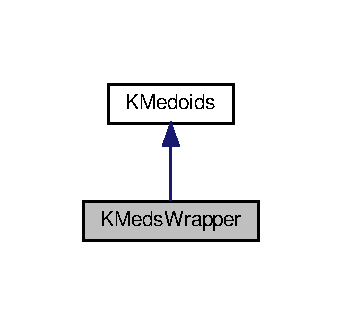
\includegraphics[width=164pt]{classKMedsWrapper__inherit__graph}
\end{center}
\end{figure}


Collaboration diagram for K\+Meds\+Wrapper\+:\nopagebreak
\begin{figure}[H]
\begin{center}
\leavevmode
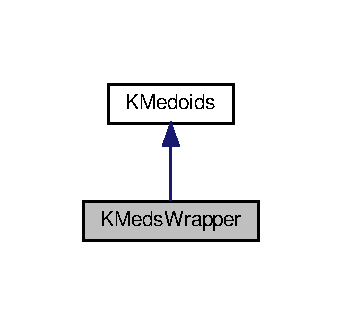
\includegraphics[width=164pt]{classKMedsWrapper__coll__graph}
\end{center}
\end{figure}
\subsection*{Public Member Functions}
\begin{DoxyCompactItemize}
\item 
void \hyperlink{classKMedsWrapper_ac0311bd5d2aef638cf794e4412426d3c}{fit\+Python} (py\+::array\+\_\+t$<$ double $>$ input\+\_\+data, std\+::string loss, int k, std\+::string log\+Filename)
\item 
py\+::array\+\_\+t$<$ double $>$ \hyperlink{classKMedsWrapper_ae825241c43b8bf92912eb59cd12ae1c5}{get\+Medoids\+Final\+Python} ()
\item 
py\+::array\+\_\+t$<$ double $>$ \hyperlink{classKMedsWrapper_af272debff6f3b31490d20b8dc7bec322}{get\+Medoids\+Build\+Python} ()
\item 
py\+::array\+\_\+t$<$ double $>$ \hyperlink{classKMedsWrapper_aba0a92e75230b7853fd533657ead656e}{get\+Labels\+Python} ()
\item 
int \hyperlink{classKMedsWrapper_a25ac2830354eeae7963cdec34d0137e8}{get\+Steps\+Python} ()
\end{DoxyCompactItemize}
\subsection*{Additional Inherited Members}


\subsection{Detailed Description}
\hyperlink{classKMedsWrapper}{K\+Meds\+Wrapper} class. Is the Python wrapper generated by Pybind that allows for calling the C++ code in Python3. 

\subsection{Member Function Documentation}
\mbox{\Hypertarget{classKMedsWrapper_ac0311bd5d2aef638cf794e4412426d3c}\label{classKMedsWrapper_ac0311bd5d2aef638cf794e4412426d3c}} 
\index{K\+Meds\+Wrapper@{K\+Meds\+Wrapper}!fit\+Python@{fit\+Python}}
\index{fit\+Python@{fit\+Python}!K\+Meds\+Wrapper@{K\+Meds\+Wrapper}}
\subsubsection{\texorpdfstring{fit\+Python()}{fitPython()}}
{\footnotesize\ttfamily void K\+Meds\+Wrapper\+::fit\+Python (\begin{DoxyParamCaption}\item[{py\+::array\+\_\+t$<$ double $>$}]{input\+\_\+data,  }\item[{std\+::string}]{loss,  }\item[{int}]{k,  }\item[{std\+::string}]{log\+Filename }\end{DoxyParamCaption})\hspace{0.3cm}{\ttfamily [inline]}}

This is the main function of the \hyperlink{classKMedoids}{K\+Medoids} module\+: this finds the build and swap medoids for the desired data


\begin{DoxyParams}{Parameters}
{\em input\+\_\+data} & Input data to find the medoids of \\
\hline
{\em loss} & The loss function used during medoid computation \\
\hline
{\em k} & The number of medoids to compute \\
\hline
{\em log\+Filename} & The name of the outputted log file \\
\hline
\end{DoxyParams}
\mbox{\Hypertarget{classKMedsWrapper_aba0a92e75230b7853fd533657ead656e}\label{classKMedsWrapper_aba0a92e75230b7853fd533657ead656e}} 
\index{K\+Meds\+Wrapper@{K\+Meds\+Wrapper}!get\+Labels\+Python@{get\+Labels\+Python}}
\index{get\+Labels\+Python@{get\+Labels\+Python}!K\+Meds\+Wrapper@{K\+Meds\+Wrapper}}
\subsubsection{\texorpdfstring{get\+Labels\+Python()}{getLabelsPython()}}
{\footnotesize\ttfamily py\+::array\+\_\+t$<$double$>$ K\+Meds\+Wrapper\+::get\+Labels\+Python (\begin{DoxyParamCaption}{ }\end{DoxyParamCaption})\hspace{0.3cm}{\ttfamily [inline]}}

This function returns the labels/medoids assignments for each datapoint after the final medoids are identified. \mbox{\Hypertarget{classKMedsWrapper_af272debff6f3b31490d20b8dc7bec322}\label{classKMedsWrapper_af272debff6f3b31490d20b8dc7bec322}} 
\index{K\+Meds\+Wrapper@{K\+Meds\+Wrapper}!get\+Medoids\+Build\+Python@{get\+Medoids\+Build\+Python}}
\index{get\+Medoids\+Build\+Python@{get\+Medoids\+Build\+Python}!K\+Meds\+Wrapper@{K\+Meds\+Wrapper}}
\subsubsection{\texorpdfstring{get\+Medoids\+Build\+Python()}{getMedoidsBuildPython()}}
{\footnotesize\ttfamily py\+::array\+\_\+t$<$double$>$ K\+Meds\+Wrapper\+::get\+Medoids\+Build\+Python (\begin{DoxyParamCaption}{ }\end{DoxyParamCaption})\hspace{0.3cm}{\ttfamily [inline]}}

This function returns the build medoids for a \hyperlink{classKMedoids}{K\+Medoids} object. \mbox{\Hypertarget{classKMedsWrapper_ae825241c43b8bf92912eb59cd12ae1c5}\label{classKMedsWrapper_ae825241c43b8bf92912eb59cd12ae1c5}} 
\index{K\+Meds\+Wrapper@{K\+Meds\+Wrapper}!get\+Medoids\+Final\+Python@{get\+Medoids\+Final\+Python}}
\index{get\+Medoids\+Final\+Python@{get\+Medoids\+Final\+Python}!K\+Meds\+Wrapper@{K\+Meds\+Wrapper}}
\subsubsection{\texorpdfstring{get\+Medoids\+Final\+Python()}{getMedoidsFinalPython()}}
{\footnotesize\ttfamily py\+::array\+\_\+t$<$double$>$ K\+Meds\+Wrapper\+::get\+Medoids\+Final\+Python (\begin{DoxyParamCaption}{ }\end{DoxyParamCaption})\hspace{0.3cm}{\ttfamily [inline]}}

This function returns the final medoids for a \hyperlink{classKMedoids}{K\+Medoids} object. \mbox{\Hypertarget{classKMedsWrapper_a25ac2830354eeae7963cdec34d0137e8}\label{classKMedsWrapper_a25ac2830354eeae7963cdec34d0137e8}} 
\index{K\+Meds\+Wrapper@{K\+Meds\+Wrapper}!get\+Steps\+Python@{get\+Steps\+Python}}
\index{get\+Steps\+Python@{get\+Steps\+Python}!K\+Meds\+Wrapper@{K\+Meds\+Wrapper}}
\subsubsection{\texorpdfstring{get\+Steps\+Python()}{getStepsPython()}}
{\footnotesize\ttfamily int K\+Meds\+Wrapper\+::get\+Steps\+Python (\begin{DoxyParamCaption}{ }\end{DoxyParamCaption})\hspace{0.3cm}{\ttfamily [inline]}}

This function returns the number of swap steps that took place during the computation 

The documentation for this class was generated from the following file\+:\begin{DoxyCompactItemize}
\item 
/home/esfrankel/\+Desktop/\+Bandit\+P\+A\+M/src/\hyperlink{kmeds__pywrapper_8cpp}{kmeds\+\_\+pywrapper.\+cpp}\end{DoxyCompactItemize}

\hypertarget{structLogHelper}{}\section{Log\+Helper Struct Reference}
\label{structLogHelper}\index{Log\+Helper@{Log\+Helper}}


Logging class for structured \hyperlink{classKMedoids}{K\+Medoids} logs.  




{\ttfamily \#include $<$kmedoids\+\_\+ucb.\+hpp$>$}

\subsection*{Public Member Functions}
\begin{DoxyCompactItemize}
\item 
void \hyperlink{structLogHelper_a8bf957fb897ae5b548264f2f614879c5}{init} (std\+::string input\+\_\+filename=\char`\"{}K\+Medoids\+Logfile\char`\"{})
\begin{DoxyCompactList}\small\item\em Opens the log file. \end{DoxyCompactList}\item 
void \hyperlink{structLogHelper_a4624149f53c4577d0565f761c155d800}{close} ()
\begin{DoxyCompactList}\small\item\em Closes the log file. \end{DoxyCompactList}\item 
void \hyperlink{structLogHelper_a5b1a8ff2ae2ce6e3293e3b34085e3b86}{write\+Summary\+Line} (std\+::string key, arma\+::rowvec vec)
\begin{DoxyCompactList}\small\item\em Writes a vector out for a given key. \end{DoxyCompactList}\item 
{\footnotesize template$<$typename T $>$ }\\void \hyperlink{structLogHelper_ad1bb80fa2bd8b1dfcd944ea19c4e8e06}{write\+Log\+String\+Line} (std\+::string key, std\+::vector$<$ T $>$ vec)
\begin{DoxyCompactList}\small\item\em Writes a logstring component. \end{DoxyCompactList}\item 
void \hyperlink{structLogHelper_a15b3f49bf98956a0585f036801e25dbe}{write\+Profile} (arma\+::rowvec b\+\_\+medoids, arma\+::rowvec f\+\_\+medoids, int steps, double loss)
\begin{DoxyCompactList}\small\item\em Writes formatted summary log of a \hyperlink{classKMedoids}{K\+Medoids} run. \end{DoxyCompactList}\end{DoxyCompactItemize}
\subsection*{Public Attributes}
\begin{DoxyCompactItemize}
\item 
\mbox{\Hypertarget{structLogHelper_a084e11845451a653f46a48ab92c97ee8}\label{structLogHelper_a084e11845451a653f46a48ab92c97ee8}} 
std\+::ofstream \hyperlink{structLogHelper_a084e11845451a653f46a48ab92c97ee8}{hlog\+File}
\begin{DoxyCompactList}\small\item\em Output stream that writes the \hyperlink{classKMedoids}{K\+Medoids} log. \end{DoxyCompactList}\item 
\mbox{\Hypertarget{structLogHelper_a7f9490e07d6bfc71b0d0fd555ca4f530}\label{structLogHelper_a7f9490e07d6bfc71b0d0fd555ca4f530}} 
std\+::vector$<$ double $>$ \hyperlink{structLogHelper_a7f9490e07d6bfc71b0d0fd555ca4f530}{comp\+\_\+exact\+\_\+build}
\begin{DoxyCompactList}\small\item\em Number of computations in build step. \end{DoxyCompactList}\item 
\mbox{\Hypertarget{structLogHelper_aaee1d830760c6b497f2fad31a0e368f8}\label{structLogHelper_aaee1d830760c6b497f2fad31a0e368f8}} 
std\+::vector$<$ double $>$ \hyperlink{structLogHelper_aaee1d830760c6b497f2fad31a0e368f8}{comp\+\_\+exact\+\_\+swap}
\begin{DoxyCompactList}\small\item\em Number of computations in swap step. \end{DoxyCompactList}\item 
\mbox{\Hypertarget{structLogHelper_a8da7e85d166977478fcfe848bb739dfa}\label{structLogHelper_a8da7e85d166977478fcfe848bb739dfa}} 
std\+::vector$<$ double $>$ \hyperlink{structLogHelper_a8da7e85d166977478fcfe848bb739dfa}{loss\+\_\+build}
\begin{DoxyCompactList}\small\item\em Loss after each iteration of build step. \end{DoxyCompactList}\item 
\mbox{\Hypertarget{structLogHelper_a3361ae9284a7fca5b867165e0380af4b}\label{structLogHelper_a3361ae9284a7fca5b867165e0380af4b}} 
std\+::vector$<$ double $>$ \hyperlink{structLogHelper_a3361ae9284a7fca5b867165e0380af4b}{loss\+\_\+swap}
\begin{DoxyCompactList}\small\item\em Loss after each iteration of swap step. \end{DoxyCompactList}\item 
\mbox{\Hypertarget{structLogHelper_aed75dac28380b3f67b777d6b36719aa9}\label{structLogHelper_aed75dac28380b3f67b777d6b36719aa9}} 
std\+::vector$<$ double $>$ \hyperlink{structLogHelper_aed75dac28380b3f67b777d6b36719aa9}{p\+\_\+build}
\begin{DoxyCompactList}\small\item\em Precision for each iteration of build step. \end{DoxyCompactList}\item 
\mbox{\Hypertarget{structLogHelper_a87a35e651ad2a32092777e1d9bd4acfa}\label{structLogHelper_a87a35e651ad2a32092777e1d9bd4acfa}} 
std\+::vector$<$ double $>$ \hyperlink{structLogHelper_a87a35e651ad2a32092777e1d9bd4acfa}{p\+\_\+swap}
\begin{DoxyCompactList}\small\item\em Precision for each iteration of swap step. \end{DoxyCompactList}\item 
\mbox{\Hypertarget{structLogHelper_a835a54928567970dd564d9eaed87597c}\label{structLogHelper_a835a54928567970dd564d9eaed87597c}} 
std\+::vector$<$ std\+::string $>$ \hyperlink{structLogHelper_a835a54928567970dd564d9eaed87597c}{sigma\+\_\+build}
\begin{DoxyCompactList}\small\item\em Distributions for each iteration of build step. \end{DoxyCompactList}\item 
\mbox{\Hypertarget{structLogHelper_afee211952d9a61c217622557e91c1275}\label{structLogHelper_afee211952d9a61c217622557e91c1275}} 
std\+::vector$<$ std\+::string $>$ \hyperlink{structLogHelper_afee211952d9a61c217622557e91c1275}{sigma\+\_\+swap}
\begin{DoxyCompactList}\small\item\em Distributions for each iteration of swap step. \end{DoxyCompactList}\end{DoxyCompactItemize}


\subsection{Detailed Description}
Logging class for structured \hyperlink{classKMedoids}{K\+Medoids} logs. 

\hyperlink{structLogHelper}{Log\+Helper} class. Assists the \hyperlink{classKMedoids}{K\+Medoids} class in structured logging. 

\subsection{Member Function Documentation}
\mbox{\Hypertarget{structLogHelper_a4624149f53c4577d0565f761c155d800}\label{structLogHelper_a4624149f53c4577d0565f761c155d800}} 
\index{Log\+Helper@{Log\+Helper}!close@{close}}
\index{close@{close}!Log\+Helper@{Log\+Helper}}
\subsubsection{\texorpdfstring{close()}{close()}}
{\footnotesize\ttfamily void Log\+Helper\+::close (\begin{DoxyParamCaption}{ }\end{DoxyParamCaption})\hspace{0.3cm}{\ttfamily [inline]}}



Closes the log file. 

Closes the log file. \mbox{\Hypertarget{structLogHelper_a8bf957fb897ae5b548264f2f614879c5}\label{structLogHelper_a8bf957fb897ae5b548264f2f614879c5}} 
\index{Log\+Helper@{Log\+Helper}!init@{init}}
\index{init@{init}!Log\+Helper@{Log\+Helper}}
\subsubsection{\texorpdfstring{init()}{init()}}
{\footnotesize\ttfamily void Log\+Helper\+::init (\begin{DoxyParamCaption}\item[{std\+::string}]{input\+\_\+filename = {\ttfamily \char`\"{}KMedoidsLogfile\char`\"{}} }\end{DoxyParamCaption})\hspace{0.3cm}{\ttfamily [inline]}}



Opens the log file. 

Opens the log file.


\begin{DoxyParams}{Parameters}
{\em input\+\_\+filename} & Filename that log will be saved as. \\
\hline
\end{DoxyParams}
\mbox{\Hypertarget{structLogHelper_ad1bb80fa2bd8b1dfcd944ea19c4e8e06}\label{structLogHelper_ad1bb80fa2bd8b1dfcd944ea19c4e8e06}} 
\index{Log\+Helper@{Log\+Helper}!write\+Log\+String\+Line@{write\+Log\+String\+Line}}
\index{write\+Log\+String\+Line@{write\+Log\+String\+Line}!Log\+Helper@{Log\+Helper}}
\subsubsection{\texorpdfstring{write\+Log\+String\+Line()}{writeLogStringLine()}}
{\footnotesize\ttfamily template$<$typename T $>$ \\
void Log\+Helper\+::write\+Log\+String\+Line (\begin{DoxyParamCaption}\item[{std\+::string}]{key,  }\item[{std\+::vector$<$ T $>$}]{vec }\end{DoxyParamCaption})\hspace{0.3cm}{\ttfamily [inline]}}



Writes a logstring component. 

Writes a logstring line for the write\+Profile function.


\begin{DoxyParams}{Parameters}
{\em key} & Key for json-\/ified output structure \\
\hline
{\em vec} & Vector to be iterated across when writing logstring line \\
\hline
\end{DoxyParams}
\mbox{\Hypertarget{structLogHelper_a15b3f49bf98956a0585f036801e25dbe}\label{structLogHelper_a15b3f49bf98956a0585f036801e25dbe}} 
\index{Log\+Helper@{Log\+Helper}!write\+Profile@{write\+Profile}}
\index{write\+Profile@{write\+Profile}!Log\+Helper@{Log\+Helper}}
\subsubsection{\texorpdfstring{write\+Profile()}{writeProfile()}}
{\footnotesize\ttfamily void Log\+Helper\+::write\+Profile (\begin{DoxyParamCaption}\item[{arma\+::rowvec}]{b\+\_\+medoids,  }\item[{arma\+::rowvec}]{f\+\_\+medoids,  }\item[{int}]{steps,  }\item[{double}]{loss }\end{DoxyParamCaption})\hspace{0.3cm}{\ttfamily [inline]}}



Writes formatted summary log of a \hyperlink{classKMedoids}{K\+Medoids} run. 

Writes summary statistics of a \hyperlink{classKMedoids}{K\+Medoids} run. Statistics include medoids after the build step, medoids after the swap step, number of swap steps, the final loss, and logstrings of the number of points that had distance computations, loss, precision, and uncertainty for each iteration of both the build and swap steps.


\begin{DoxyParams}{Parameters}
{\em b\+\_\+medoids} & Medoids after the build step. \\
\hline
{\em f\+\_\+medoids} & Medoids after the swap step (final medoids). \\
\hline
{\em steps} & Number of swap steps. \\
\hline
{\em loss} & Final loss of the \hyperlink{classKMedoids}{K\+Medoids} object. \\
\hline
\end{DoxyParams}
\mbox{\Hypertarget{structLogHelper_a5b1a8ff2ae2ce6e3293e3b34085e3b86}\label{structLogHelper_a5b1a8ff2ae2ce6e3293e3b34085e3b86}} 
\index{Log\+Helper@{Log\+Helper}!write\+Summary\+Line@{write\+Summary\+Line}}
\index{write\+Summary\+Line@{write\+Summary\+Line}!Log\+Helper@{Log\+Helper}}
\subsubsection{\texorpdfstring{write\+Summary\+Line()}{writeSummaryLine()}}
{\footnotesize\ttfamily void Log\+Helper\+::write\+Summary\+Line (\begin{DoxyParamCaption}\item[{std\+::string}]{key,  }\item[{arma\+::rowvec}]{vec }\end{DoxyParamCaption})\hspace{0.3cm}{\ttfamily [inline]}}



Writes a vector out for a given key. 

Writes a vector out for a given key


\begin{DoxyParams}{Parameters}
{\em key} & Key for json-\/ified output structure \\
\hline
{\em vec} & Vector to be iterated across when writing line \\
\hline
\end{DoxyParams}


The documentation for this struct was generated from the following file\+:\begin{DoxyCompactItemize}
\item 
/home/esfrankel/\+Desktop/\+Bandit\+P\+A\+M/headers/kmedoids\+\_\+ucb.\+hpp\end{DoxyCompactItemize}

\chapter{File Documentation}
\hypertarget{kmedoids__ucb_8cpp}{}\doxysection{/\+Users/dhavaldangaria/\+Bandit\+PAM/src/kmedoids\+\_\+ucb.cpp File Reference}
\label{kmedoids__ucb_8cpp}\index{/Users/dhavaldangaria/BanditPAM/src/kmedoids\_ucb.cpp@{/Users/dhavaldangaria/BanditPAM/src/kmedoids\_ucb.cpp}}
{\ttfamily \#include \char`\"{}kmedoids\+\_\+ucb.\+hpp\char`\"{}}\newline
{\ttfamily \#include $<$carma.\+h$>$}\newline
{\ttfamily \#include $<$armadillo$>$}\newline
{\ttfamily \#include $<$unordered\+\_\+map$>$}\newline
{\ttfamily \#include $<$regex$>$}\newline
Include dependency graph for kmedoids\+\_\+ucb.\+cpp\+:
\nopagebreak
\begin{figure}[H]
\begin{center}
\leavevmode
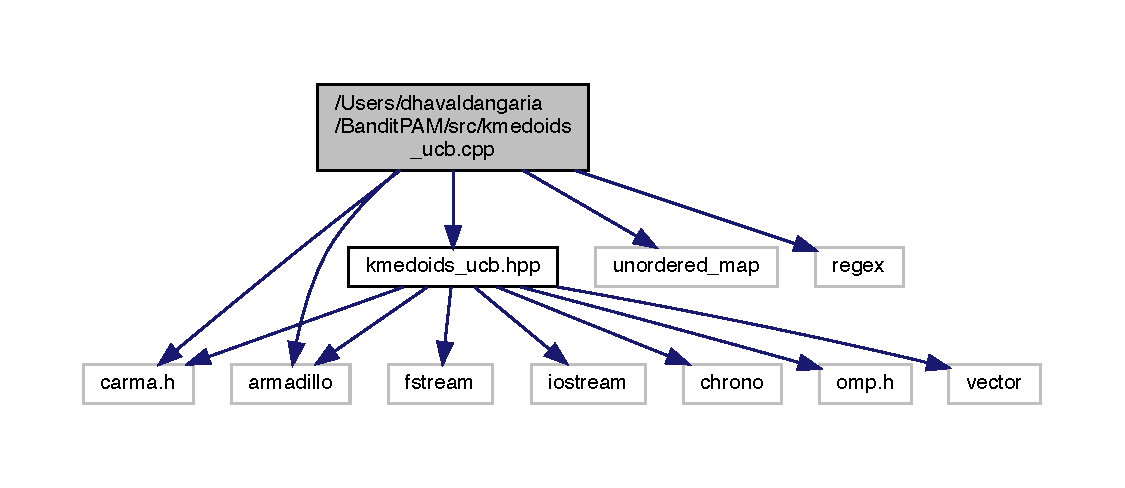
\includegraphics[width=350pt]{kmedoids__ucb_8cpp__incl}
\end{center}
\end{figure}


\doxysubsection{Detailed Description}
\begin{DoxyDate}{Date}
2020-\/06-\/10
\end{DoxyDate}
This file contains the primary C++ implementation of the Bandit\+PAM code. 

\hypertarget{kmeds__pywrapper_8cpp}{}\section{/home/esfrankel/\+Desktop/\+Bandit\+P\+A\+M/src/kmeds\+\_\+pywrapper.cpp File Reference}
\label{kmeds__pywrapper_8cpp}\index{/home/esfrankel/\+Desktop/\+Bandit\+P\+A\+M/src/kmeds\+\_\+pywrapper.\+cpp@{/home/esfrankel/\+Desktop/\+Bandit\+P\+A\+M/src/kmeds\+\_\+pywrapper.\+cpp}}
{\ttfamily \#include $<$armadillo$>$}\newline
{\ttfamily \#include $<$carma/carma.\+h$>$}\newline
{\ttfamily \#include $<$pybind11/pybind11.\+h$>$}\newline
{\ttfamily \#include $<$pybind11/numpy.\+h$>$}\newline
{\ttfamily \#include \char`\"{}kmedoids\+\_\+ucb.\+hpp\char`\"{}}\newline
Include dependency graph for kmeds\+\_\+pywrapper.\+cpp\+:\nopagebreak
\begin{figure}[H]
\begin{center}
\leavevmode
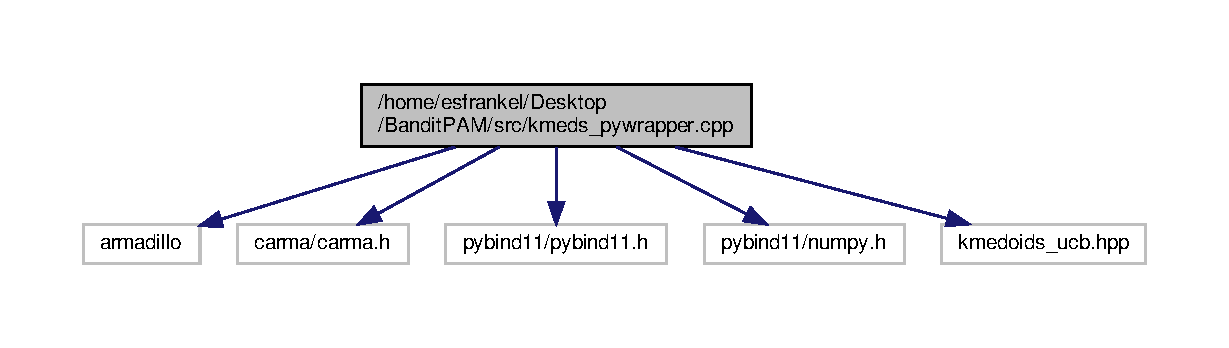
\includegraphics[width=350pt]{kmeds__pywrapper_8cpp__incl}
\end{center}
\end{figure}
\subsection*{Classes}
\begin{DoxyCompactItemize}
\item 
class \hyperlink{classKMedsWrapper}{K\+Meds\+Wrapper}
\begin{DoxyCompactList}\small\item\em Python wrapper for \hyperlink{classKMedoids}{K\+Medoids} class. \end{DoxyCompactList}\end{DoxyCompactItemize}
\subsection*{Functions}
\begin{DoxyCompactItemize}
\item 
\mbox{\Hypertarget{kmeds__pywrapper_8cpp_a66c5e3323d71e29a0a148bec731ac27b}\label{kmeds__pywrapper_8cpp_a66c5e3323d71e29a0a148bec731ac27b}} 
{\bfseries P\+Y\+B\+I\+N\+D11\+\_\+\+M\+O\+D\+U\+LE} (Bandit\+P\+AM, m)
\end{DoxyCompactItemize}


\subsection{Detailed Description}
\begin{DoxyDate}{Date}
2020-\/06-\/10
\end{DoxyDate}
Creates the Python bindings for the C++ code that allows it to be called in Python. 
\hypertarget{main_8cpp}{}\doxysection{/\+Users/motiwari/\+Desktop/\+Bandit\+PAM/src/main.cpp File Reference}
\label{main_8cpp}\index{/Users/motiwari/Desktop/BanditPAM/src/main.cpp@{/Users/motiwari/Desktop/BanditPAM/src/main.cpp}}
{\ttfamily \#include \char`\"{}kmedoids\+\_\+algorithm.\+hpp\char`\"{}}\newline
{\ttfamily \#include $<$armadillo$>$}\newline
{\ttfamily \#include $<$chrono$>$}\newline
{\ttfamily \#include $<$fstream$>$}\newline
{\ttfamily \#include $<$unistd.\+h$>$}\newline
{\ttfamily \#include $<$exception$>$}\newline
{\ttfamily \#include $<$regex$>$}\newline
{\ttfamily \#include $<$filesystem$>$}\newline
Include dependency graph for main.\+cpp\+:
\nopagebreak
\begin{figure}[H]
\begin{center}
\leavevmode
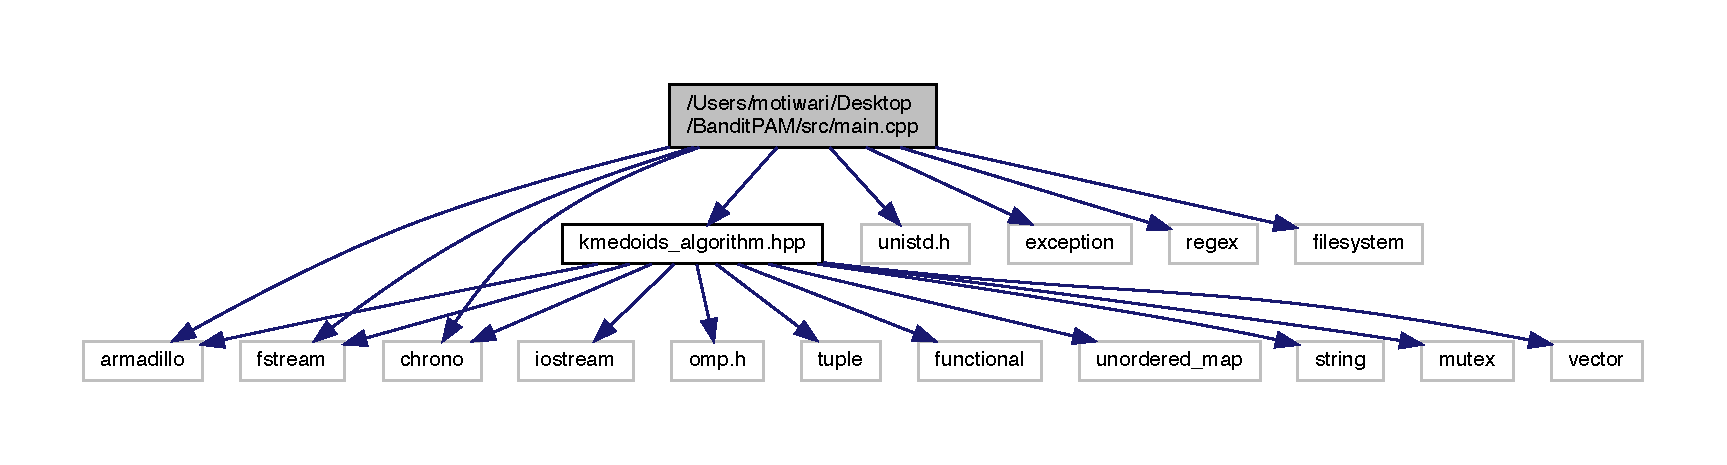
\includegraphics[width=350pt]{main_8cpp__incl}
\end{center}
\end{figure}
\doxysubsection*{Functions}
\begin{DoxyCompactItemize}
\item 
\mbox{\Hypertarget{main_8cpp_a0ddf1224851353fc92bfbff6f499fa97}\label{main_8cpp_a0ddf1224851353fc92bfbff6f499fa97}} 
int {\bfseries main} (int argc, char $\ast$argv\mbox{[}$\,$\mbox{]})
\end{DoxyCompactItemize}


\doxysubsection{Detailed Description}
\begin{DoxyDate}{Date}
2020-\/06-\/10
\end{DoxyDate}
Defines a command line program that can be used to run the \mbox{\hyperlink{classBanditPAM}{Bandit\+PAM}} KMedoids algorithm.

Usage (from home repo directory)\+: ./src/build/\+Bandit\+PAM -\/f \mbox{[}path/to/input\mbox{]} -\/k \mbox{[}number of clusters\mbox{]} 

%--- End generated contents ---

% Index
\backmatter
\newpage
\phantomsection
\clearemptydoublepage
\addcontentsline{toc}{chapter}{Index}
\printindex

\end{document}
